\documentclass{article}
\usepackage{amsmath}
\usepackage{amssymb}
\usepackage{graphicx}
\usepackage{hyperref}
\usepackage[version=4]{mhchem}

\title{Example 2}
\date{}

\begin{document}
\maketitle

(AMC) In triangle \(A B C, B D\) is a median. \(C F\) intersects \(B D\) at \(E\) so \(B E\) \(=E D\). Point \(F\) is on \(A B\). Then, if \(B F=5, B A\) equals:\\
(A) 10\\
(B) 12\\
(C) 15\\
(D) 20\\
(E) none of these

Solution: (C).\\
\centering
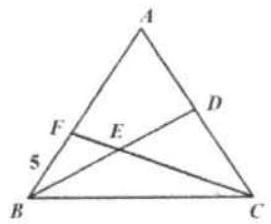
\includegraphics[width=\textwidth]{images/102(4).jpg}

Method 1:\\
Draw \(D G / / A B\) to meet \(C F\) at \(G\). Since \(D\) is the midpoint of \(A C\),


\(A F=2 D G\).\\
Since \(B E=E D, \angle E B F=\angle E D G\) (alternate interior angles) and \(\angle B E F=\angle D E G\) (vertical angles),\\
\(\triangle E F B \cong \triangle E G D\) and \(D G=B F=5\).\\
\centering
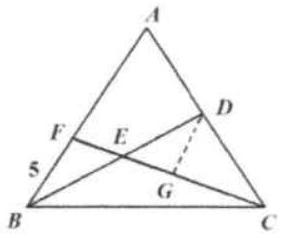
\includegraphics[width=\textwidth]{images/103(1).jpg}\\
\(A F=2 D G=10 . A B=5+10=15\).

Method 2:\\
Draw \(D G / / C F\) to meet \(A B\) at \(G\). Since \(D\) is the midpoint of \(A C\), \(A G=G F\).\\
Since \(D G / / E F\), and \(E\) is the midpoint of \(B D\),\\
\centering
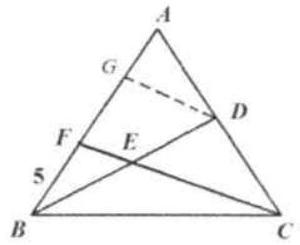
\includegraphics[width=\textwidth]{images/103(2).jpg}\\
\(G F=B F\).

So \(A G=G F=B F=5\).\\
\(A B=B F+F G+A G=5+5+5=15\).

Method 3:\\
Draw \(E G / / A C\) to meet \(A B\) at \(G\). Since \(E\) is the midpoint of \(B D\),\\
\(A B=2 A G=2 B G=2 y=5+x+y \Rightarrow y=5+x\)

Since \(E G / / A C, \triangle F A C \sim \triangle F G E\) and\\
\((x+y) / x=4 \Rightarrow y=3 x\)\\
Substituting (2) into (1): \(3 x=5+x \Rightarrow 2 x=5\)\\
\centering
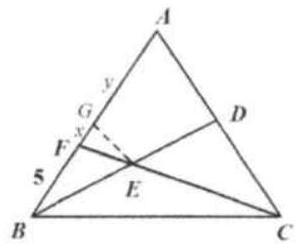
\includegraphics[width=\textwidth]{images/103(6).jpg}

So \(A B=2 y=10+2 x=10+5=15\).

Note: the following ways to draw the auxiliary line will not work.\\
\centering
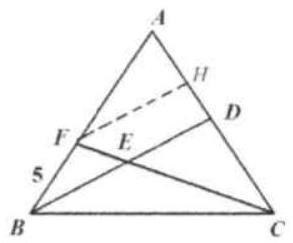
\includegraphics[width=\textwidth]{images/103.jpg}\\
\(F H / / B D\)\\
\centering
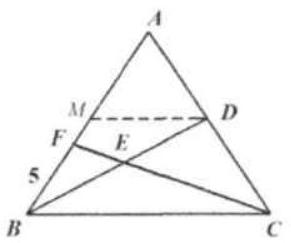
\includegraphics[width=\textwidth]{images/103(5).jpg}\\
\(D M / / B C\)\\
\centering
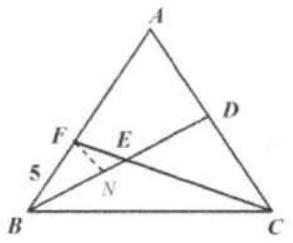
\includegraphics[width=\textwidth]{images/103(4).jpg}\\
\(F N / / A C\)\\
\centering
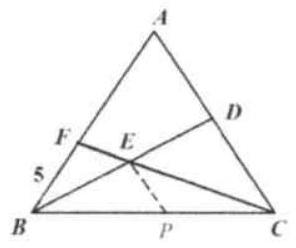
\includegraphics[width=\textwidth]{images/103(3).jpg}

EP // AC



\end{document}
